\documentclass{../templates/topic}

\begin{document}
\graphicspath{{assets/}{ch3_Time_Domain_Performance_Characteristics/assets/}}

\chapter{Transient Response Characteristics}

\begin{section}{Definitions}
	
	All of these refer in general to the Unit Step Response.
	
	\definition{rise time $\approx \frac{1.8}{\omega_n}$}  time from a percentage from the initial values to the 1st time encountering a percentage from the final value. Most commonly, it is from 0.1 of initial to 0.9 of final.
	
	\definition{peak time $\approx \frac{\pi}{\omega_d}$}  time to hit the highest value. More generally, the time until the first peak.
	
	\definition{settling time $\approx \frac{4}{\zeta\omega_n} (for 0.02)$}  time before the system has converged to within a specified percentage of the final value.
	
	\definition{overshoot $ \approx \exp[\frac{-\pi\zeta}{\sqrt{1-\zeta^2}}] $} ratio of the height of the 1st peak above the final value to the final value.
	
	\begin{figure}[H]
		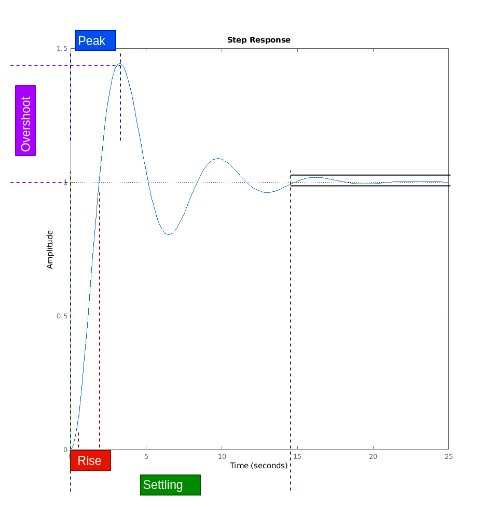
\includegraphics[width=\textwidth]{characteristics_on_graph.png}
		\caption{Time Response Characteristics on a sample function}
	\end{figure}
	
\end{section}

\begin{section}{Designing for Characteristics}
	\subsection{Overshoot}
		\begin{equation*}
			\zeta = \sqrt{\frac{(\ln{M_p})^2}{\pi^2+(\ln{M_p})^2}}
		\end{equation*}
	
\end{section}

\end{document}